\documentclass[10pt, a4paper]{article}
\usepackage{lrec2006}

\usepackage[english]{babel}
\usepackage{ucs}
\usepackage[utf8x]{inputenc}
%\usepackage[dvips]{graphicx}
\usepackage{graphicx}
\usepackage{url}
\usepackage{latexsym}
\usepackage{lingmacros} % for enumsentence
\usepackage{mdwlist}

% 4-8 pages (let's keep it as short as possible)
% cite==cite  citeyear==newcite

\title{TIMEN: An Open Temporal Expression Normalisation Resource}


\name{Hector Llorens$^{\ast}$, Leon Derczynski$^{\dagger}$, Robert Gaizauskas$^{\dagger}$, Estela Saquete$^{\ast}$}
\address{$^{\ast}$University of Alicante\\ 03690, Spain\\ \texttt{{hllorens,stela}@dlsi.ua.es} \\ \\
         $^{\dagger}$University of Sheffield\\ S1 4DP, UK\\ \texttt{{leon,robertg}@dcs.shef.ac.uk}}

         
\abstract{Temporal expressions are words or phrases that describe a point, duration or recurrence in time. Automatically annotating these expressions is a research goal of increasing interest. Recognizing them can be achieved with minimally supervised machine learning, but interpreting them accurately (normalisation) is a complex task requiring human knowledge.
In this paper, we present TIMEN, a community-driven tool for temporal expression normalisation. 
TIMEN is derived from current best approaches and is an independent tool,
enabling easy integration in existing systems.
We argue that temporal expression normalisation can only be effectively performed with a large knowledge base and set of rules. Our solution is a framework and system with which to capture this knowledge for different languages. Using both existing and newly-annotated data, we present results showing competitive performance and invite the IE community to contribute to a knowledge base in order to solve the temporal expression normalisation problem.
\\ \newline
\Keywords{Temporal Information Processing, TimeML, timex normalisation, ISO 8601, Open Resource}
}



\begin{document}

\maketitleabstract

\section{Introduction}

This paper addresses temporal expression processing in natural language, which is framed in the field of information extraction (IE). We present an open, extensible and state-of-the-art temporal normalisation library TIMEN (\texttt{http://www.timen.org/}), that improves upon all other publicly-available system performances.

A temporal expression (or \textbf{timex}) is a linguistic expression referring to a time, period, or recurring pattern in time (for example \emph{``next month"}, \emph{``3~hours"}, \emph{``weekly"}). Timex annotation involves the recognition of these expressions and then their interpretation, resulting in an encoded annotation of the timex's semantics. This interpretation task is called \textbf{timex normalisation}.

The comprehension of temporal expressions is critical to accurate processing of discourse semantics. Achieving this has been a long-standing research task~\cite{Mani2000,Verhagen2010-TempEval-2}. Aside from the intrinsic value it has in understanding discourse semantics, temporal information is crucial for information processing tasks including question answering~\cite{Saquete2009a}, text summarisation~\cite{Daniel2003}, information retrieval~\cite{Baeza-Yates2007TimeIR}, and knowledge base population~\cite{ji2011kbp}.

Recognizing timexes can be performed using machine learning and has been achieved with relatively simple feature sets~\cite{Llorens2011-Dynamic-Window}.
However, any practical approach to timex normalisation requires a hand-crafted rule set. The scale of annotated data and intelligent reasoning required to automatically infer, for example, the rules about the date of Easter Sunday, the associations between hemisphere and seasons or the dates of Chinese Spring Festival is too large.

Previous approaches to timex normalisation have included their own custom rule sets and typically reach 60\%-90\% accuracy depending on evaluation dataset.
Scant efforts have been made to build upon prior systems' performance. Instead each system has incorporated a new, unique built-in rule set that captures a majority of timex instances (for a given training set) which are accounted for by a limited range of timex texts. This performance cap demonstrates the inherent disadvantages of rule-based approaches. Closed, integrated or proprietary rule bases are not equipped to normalise unseen timexes at all, or to grow in order to handle them.

Further, much of the normalisation effort is inherently language-independent, working with structures such as calendars and simple temporal constructs such as month and day names. Separating logic for dealing with this from language-specific requirements enables effective normalisation across languages.

The sparsity of temporally annotated training data and its confinement to the newswire genre suggest that the real accuracy rate of existing systems will be lower than their evaluation indicates.
In light of this, our overall research question is: How can we reach 100\% normalisation accuracy in timex interpretation? We accept that achieving maximum accuracy may be complex and time-consuming and that some unconquerable errors may be caused by poor-quality input documents. Towards this goal, the questions we answer in this paper are as follows:

\begin{enumerate}
\item How can we create a high-performance multi-lingual timex normalisation system? E.g. how will we normalise timexes in a way that improves upon prior work?
\item How can a normalisation system be made permanent, reusable and extensible? That is, what features must a normalisation system have so that it can grow over time? 
\end{enumerate} 

To address the first we propose an approach involving hand-crafted rules and a custom rule processing engine. This builds on various rule sets extracted or intuited from previous systems and includes a performance evaluation component. 

In response to the second, we propose a rule creation strategy that includes a constant performance evaluation component and is driven by corpus-based failure analysis. This is openly accessible via a community editable rule base. 

The remainder of our paper is as follows. In Section~\ref{background}, we provide descriptions of timexes according to modern standards and summarise previous approaches to timex normalisation. We describe our system in Section~\ref{overview} and present a comparative evaluation of state-of-the-art timex normalisation systems in Section~\ref{evaluation}, before concluding.


\section{Background}
\label{background}

\subsection{Temporal Expressions and Normalisation}
Timex processing consists of recognizing temporal expressions in text, as well as classifying and normalising them.
This normalisation subtask consists of obtaining the absolute value of a timex regardless of the linguistic expression used. The normalisation of two timexes is shown in Example~\ref{ex-timex}.

\small
\enumsentence{
a. He was born in \underline{June 1983}$_{1983-06}$.\\
b. He was born in \underline{06/1983}$_{1983-06}$.\\
%\vspace{-0.4cm}
}\label{ex-timex}
\normalsize

The timexes underlined in (\ref{ex-timex}a) and (\ref{ex-timex}b) normalise to the same value (\textit{1983-06}). 
All semantically equivalent timexes encode to the same value.


Currently, the standard temporal annotation scheme is TimeML\footnote{See \url{http://timeml.org/}.}~\cite{Pustejovsky2003TimeML}, which includes a specification of the TIMEX3 standard.
According to this scheme, the normalised value of a timex must be expressed in one of the following notations: (i) a Gregorian calendar time or date formatted in the ISO 8601 standard as in~(\ref{E-ISO8601}a), or (ii) a period formatted as \texttt{P}, a \texttt{number} and an abbreviated \texttt{temporal unit} as in~(\ref{E-ISO8601}b). 

\small
\enumsentence{a. October 2012: \texttt{2012-10}\\b. Two weeks: \texttt{P2W}\\\vspace{-0.4cm}
}\label{E-ISO8601}
\normalsize

The complexity of the task comes from the variability of language for expressing time and also the fact that there are timexes whose accurate interpretation depends on other time references, the current tense and various linguistic features -- see Example~(\ref{relative}).

\small
\enumsentence{a. Monday\\b. two days after}\label{relative}
\normalsize

In~(\ref{relative}a), we need the utterance or document creation time (DCT) and the tense to obtain the normalised value. In~(\ref{relative}b), we need to refer to a previously-mentioned temporal expression to perform normalisation.


\subsection{Timex Normalisation Taxonomy}

One of the key points of the task is the taxonomy of the different timexes regarding how these are normalised.
Most of the approaches coincide that timexes can be:

\begin{itemize}
\item \textbf{Explicit, absolute, or self-contained}: These can be directly translated to a particular granularity date/time.
\item \textbf{Implicit, relative, or context-dependent}: These need the document creation time (deictic) or a previously mentioned temporal reference/anchoring (anaphoric) to obtain a explicit date/time.
\item \textbf{Durative}: Describing a bounded interval (or duration) that is not inherently anchored to a timeline.
\item \textbf{Set or frequency}: Regularly recurring times, such as \emph{``every Christmas"} or \emph{``each Tuesday"}.
\item \textbf{Vague}: generic mentions like \emph{``recently"} or \emph{``today"} in \emph{``today's fashions"}; see TIDES standard Section~4.6~\cite{Ferro2005TIDES}.
\end{itemize}

The information and reasoning required to type and interpret temporal expressions is complex. One must rely on contextual clues, world knowledge and discourse anaphora in order to correctly perform timex normalisation.


\subsection{Previous Work}
\label{previous}

There have been many previous approaches to the timex normalisation task. We will describe older TIMEX2 systems which laid the foundation of timex normalisation, and then state-of-the-art systems and those involved in TempEval-2.

%We group the systems listed below according to their approach and provide a brief comparison of normalisation performances. The systems are:

%\begin{itemize*}
%\item TempEx-GUTime~\cite{Mani2000,Verhagen2005TARSQI}
%%Schilder and Habel \shortcite{Schilder-Habel2001-From-timex-to-complete-temporal-info-German}, 
%\item Chronos~\cite{Negri2004TERN}
%\item TERSEO~\cite{Saquete2006TERSEO}
%\item TimexTag~\cite{Ahn2005-CRF}
%\item TEA~\cite{Han-Levin2006-TEA}
%\item DANTE~\cite{Mazur-Dale2007-DANTE}
%\item USFD2~\cite{Derczynski2010-TempEval2-USFD2}
%\item TERNIP~\cite{ternip}
%\item HeidelTime~\cite{Strotgen2010-TempEval2-Heidel}
%\item TRIPS/TRIOS~\cite{UzzamanAllen2010-TempEval2-TRIPS-TRIOS}
%\item TIPSem~\cite{Llorens2010TempEval-2}.
%\end{itemize*}

\subsection{Pre-TIMEX3}

One of the first relevant approaches to the normalisation task was TempEx \cite{Mani2000} more recently implemented as GUTime \cite{Verhagen2005TARSQI}. This was an early proposal to the robust temporal processing of news. It defined an annotation scheme and a system to recognize and normalise timexes excluding durations (e.g., \emph{``two years''}), generics (e.g., \emph{``today's youth''}) and fuzzy expressions (e.g., \emph{``few months ago''}). In the normalisation they distinguished explicit (self-contained or SC) and implicit (context-dependent or DP) timexes.
Furthermore, within the implicit ones they differentiate those relative to the DCT and those relative to a previously mentioned timex (\textit{temporal focus}). For normalising, this system uses the following features relative to a timex: words, part-of-speech (PoS) the reference time (DCT or focus), governing tense and governing prepositions (also known as temporal signals).


%Schilder and Habel \citeyear{Schilder-Habel2001-From-timex-to-complete-temporal-info-German} defined a taxonomy consisting of explicit, implicit (indexical) and vague (fuzzy) timexes. The features used by this system are the same plus expressions granularity. This gives information about the granularity of both absolute and relative expressions in such a way that if a relative expression needs to find its anchor their granularity must be compatible.

In the TERN 2004 evaluation, the Chronos system~\cite{Negri2004TERN} reached the highest performance.
 This system followed the TIMEX2\footnote{See \url{http://fofoca.mitre.org/}.} annotation guidelines.
Similar to GUTime, the approach differentiated absolute and relative timexes. Again, these were divided into those relative to DCT and those relative to a previous temporal reference.

TERSEO \cite{Saquete2006TERSEO} is a later TIMEX2 system that improves upon Chronos. It accounts for period and fuzzy expressions. The system includes a FOL-based rule syntax and a method to automatically extend rules to other languages.

DANTE \cite{Mazur-Dale2007-DANTE} also uses rules and follows TIMEX2. The timexes it can process can be fully specified, implicit-underspecified  (e.g., \emph{``April 2nd''}), implicit-relative (e.g., \emph{``3 days ago''}), duration or frequency/set expressions. The differentiation of underspecified timexes and the definition of their local semantics is the main contribution of this work. Unfortunately, the system is not publicly available.

TimexTag \cite{Ahn2005-CRF} is another rule-based approach to normalisation which follows TIMEX2 specifications. This defines a taxonomy consisting of points, which include explicit, deictic (relative to DCT) and anaphoric (relative to previous reference) timexes, durations, vague points (e.g., \emph{``in the past''}) and recurrences (e.g., \emph{``each Sunday''}). They define a pattern or regular expression based rule syntax for the different s.pdf of their normalisation process. TEA \cite{Han-Levin2006-TEA} uses rules but follows the recent TIMEX3 standard. This classifies timexes in explicit, deictic (relative to DCT), relative (relative to previous references) and duration. This work includes a self-implemented Gregorian calendar model and a time calculus strategy. They define a formal and expressive rule syntax based on their time calculus. Both TimexTag and TEA rely on hierarchical constraint satisfaction.

\subsection{State of the art}

Recently, systems have focused on the TIMEX3 standard included with TimeML. The most current direct performance comparison is the TempEval-2 evaluation exercise~\cite{Verhagen2010-TempEval-2}. All the best systems in the typing and normalisation tasks were rule-based.

USFD2 \cite{Derczynski2010-TempEval2-USFD2} was a minimal system, with only seven rules. While achieving a high TIMEX3 typing accuracy (90\%), the more complex normalisation task was very difficult for such a system

HeidelTime \cite{Strotgen2010-TempEval2-Heidel} performed recognition and normalisation with rules, and catered for explicit, durative, implicit (relative to DCT), and relative timexes. Its regex-based rules use an internal symbol set encoding for temporal concepts such as months and calendar events. This system had the best normalisation performance over the TempEval-2 expressions that it recognised (85\%).

TRIPS/TRIOS \cite{UzzamanAllen2010-TempEval2-TRIPS-TRIOS} had a data-driven recognition component, with rule-based timex typing and normalisation. The normlisation part is a pattern/RE based algorithm which is publicly available on-line.

TIPSem \cite{Llorens2010TempEval-2} implemented a hybrid strategy for normalisation. Firstly a learned classifier determines the normalisation type (explicit, relative to DCT, relative to previous reference, duration, set or vague). Then, handcrafted rules based on pattern matching are applied depending on normalisation type.

Finally, although not part of the TempEval-2 exercise, TERNIP~\cite{ternip} is a modern re-implementation of GUTime, using a system-independent rule base and sophisticated syntax. TERNIP is designed for modular extension and use in temporal evaluation tasks.

From the described systems, the following are publicly available and will work with TIMEX3-annotated TimeML: TERNIP\footnote{\scriptsize \url{https://github.com/cnorthwood/ternip}} (based on GUTime), TIPSem\footnote{\scriptsize \url{http://gplsi.dlsi.ua.es/demos/TIMEE}}, and HeidelTime\footnote{\scriptsize \url{http://dbs-projects.ifi.uni-heidelberg.de}}. Therefore, these are the systems to which we will compare TIMEN (see Section~\ref{evaluation}).


\section{TIMEN Overview}
\label{overview}

We introduce our approach in this section. The overall operation of TIMEN is as follows. Firstly, the string to be normalised is taken, with some contextual information. Next this is converted into a symbolic representation using a knowledge base. Rules are then matched against the representation. Finally, a normalised output is produced in TIMEX3 format. These are detailed below as we discuss the core functionality of the system and how we manage collaboration.

The distinguishing characteristics of TIMEN are independence from other timex processing tasks, an open philosophy and multilinguality. The architecture of TIMEN clearly separates: (i) the algorithms (source code) which conduct the task and (ii) the knowledge and rules necessary for the process.

\subsection{TIMEN Library}

We developed TIMEN as a resource that outputs a timex's normalised value given a timex, a set of features and an input language.
TIMEN takes a timex, a DCT, a date\_ref, and a tense as input and outputs the corresponding normalised value according to the TIMEX3 standard.
To obtain the normalised value it makes use of the knowledge database (knowledge base) and the rule database (rulebase).
To better explain the processing flow of TIMEN, we describe an example.

%TIMEN has been developed as a Java library to give freedom to the final users on how to integrate it to their systems or projects, and how to handle the context which will be explained afterwards.
%Figure~\ref{fig:TIMEN} summarizes the architecture of TIMEN.

\begin{figure}[htbp]
 \begin{center}
  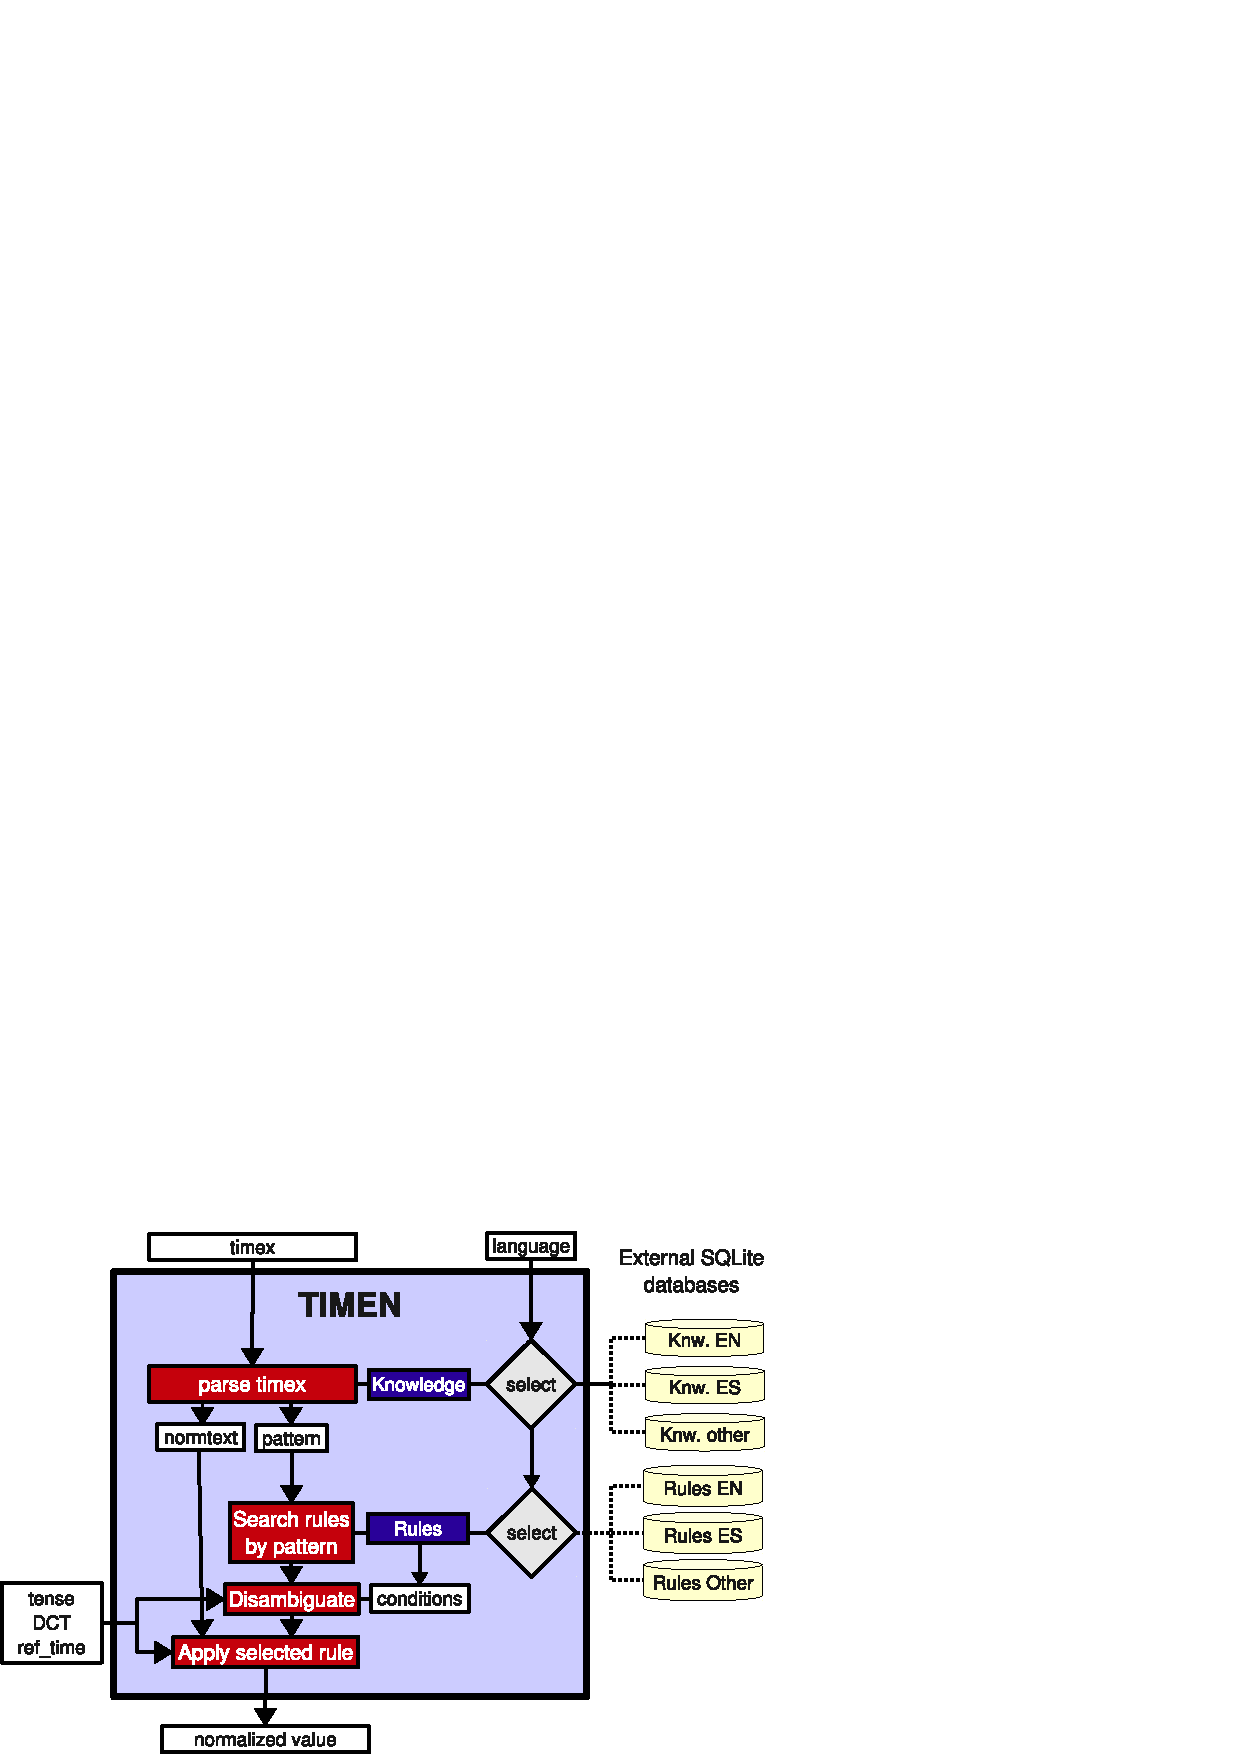
\includegraphics[width=0.5\textwidth,clip]{eps/TIMEN-architecture-TIMEN-detail.pdf}
  \caption{TIMEN Architecture}
  \label{fig:TIMEN}
  \end{center}
\end{figure}


\subsubsection{Input Data}
Consider that we run TIMEN with the following input data: text of \texttt{October 25}, DCT is 2012-02-02, reference time of 2012-02-01, the phrase in the past tense, and the language is English. 

\subsubsection{Symbolic Representation}

Firstly, TIMEN parses the timex using the English knowledge base (\textbf{KB} -- see Section~\ref{kb}) to obtain a normalised text (normtext) and a pattern, which is the original text with certain phrases -- such as weekday names -- converted to language independent symbols.

The pattern is used to match rules in the rulebase, and the normtext is used to obtain the final normalised value from a simplified text (e.g., always in lower case, spelled numbers are translated to numbers, tokenisation where \texttt{\_} is the separator).

\textbf{Example:}
For \textit{October 25}, the pattern is \textit{TMonth\_Num}. This would be the same for any month followed by a number (e.g., Mar 1999).

For \textit{October 25}, the normtext is \textit{october\_25}.

\subsubsection{Rule Matching}
The next step is querying the rulebase with the pattern obtained. For the pattern \textit{TMonth\_Num} we might find two rules: one for expressions representing a month followed by a day and another for those representing a month followed by a year.

\textbf{Example:}
Since we matched more than one rule we need to select which one of them to apply. In order to select the rule, TIMEN follows a disambiguation process.
This consists of checking in order if the found rules have conditions and if so checking whether normtext matches them. The first rule found that matches the conditions (or does not have conditions) is applied.

In the current TIMEN rulebase, we find two rules for \textit{TMonth\_Num}. The first one refers to a month followed by a day and has the condition token(1)$<$32, which means that the word in position 1 (starting by 0) of normtext is a number and it is lower than 32. The second one refers to a month followed by a year and has no conditions. Since the rules are retrieved in order the first one will be always checked before the second.

For \textit{october\_25}, the condition of the first rule is matched and then TIMEN will apply the rule to obtain the normalisation of a month followed by a day \textit{DATE\_MONTH\_DAY(DCT,token(0),token(1))}.

\subsubsection{TIMEX3 Output}
In order to apply the matched rule TIMEN will use the rule, the symbolic representation of the input text, and the supplied input features.

\textbf{Example:}
Information required at this point is tense, DCT and the values \textit{october} and \textit{25}. In this case, since the tense is past and the DCT is set to 2nd of February, the normalised output will be \textit{2011-10-25}.

\subsubsection{Discourse Management}
Below in the subsection dedicated to the knowledge base and the rulebase we better explain the elements of the patterns and the syntax of the rules\footnote{\scriptsize A complete technical reference to the knowledge base and rule syntax, as well as the syntax of rule conditions, is described at \url{http://timen.org/}.}.

Since TIMEN is just a library we need an application which uses it. In order to give to final users an example application we developed TIMEN\_CONSUMER.

\subsection{Using TIMEN}

Applying TIMEN to task of normalised TIMEX3s in text requires some extra work. To this end, in this section we introduce TIMEN\_CONSUMER, which handles discourse-level information and document processing for TIMEN.

TIMEN\_CONSUMER is an example application developed to show how to integrate TIMEN in major projects.
TIMEN\_CONSUMER aims to perform timex normalisation in two basic situations:

\begin{enumerate}
\item There is a timex without any context (e.g., \emph{``October"}) and you want to know its normalised value.
\item There is a TimeML file where DCT and timexes are annotated and you want to add or update the normalisation values of the timexes.
\end{enumerate}

As discussed above, a timex often cannot be normalised in isolation -- contextual information such as temporal references and the tense of the verbs governing the timexes is often required. The best dataset for comparison to similar systems is the TempEval-2 set, which also consists of scenarios involving contextual information. Therefore, to demonstrate the benefits of TIMEN over prior timex processing systems, we focus on the second situation.

Figure \ref{fig:arch} shows the architecture of TIMEN\_CONSUMER integrating the TIMEN library.

\begin{figure}[htbp]
 \begin{center}
  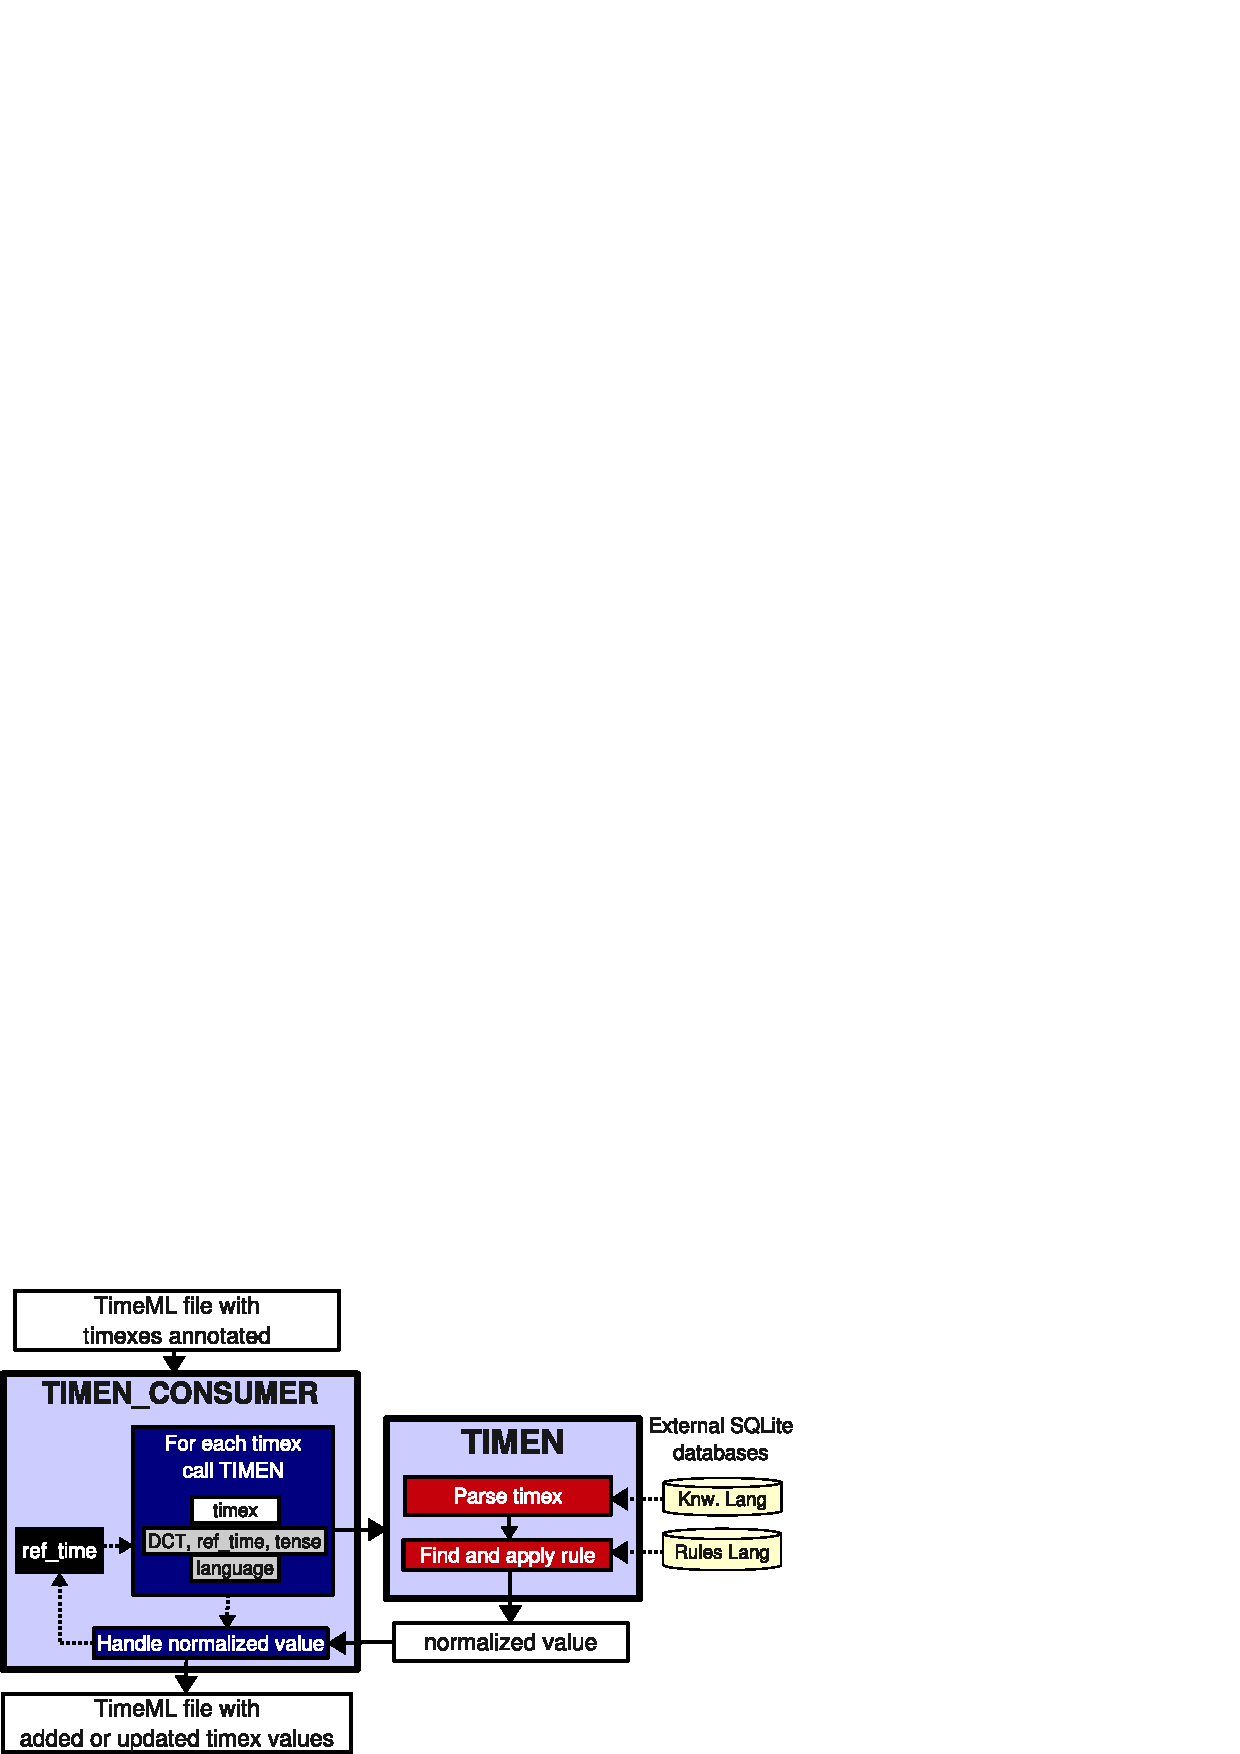
\includegraphics[width=0.5\textwidth,clip]{eps/TIMEN-architecture-supersimple.pdf}
  \caption{Architecture Overview}
  \label{fig:arch}
  \end{center}
\end{figure}


TIMEN\_CONSUMER controls discourse-level information, saving previously normalised timexes in order to track reference time~\cite{Reichenbach1947-Tense} and also handling tenses which affect timexes.
It takes a TimeML document containing delimited timexes as input and manages their presentation to the TIMEN library, which generates normalisations. Because TIMEN is available as a decoupled library, anyone may implement their own wrapper strategy for handling context; TIMEN\_CONSUMER is provided as an example, to allow rapid standalone normalisation.



\subsection{Knowledge Base and Rules}
\label{kb}

TIMEN relies on external knowledge, stored as symbolic or axiomatic representations. Here we describe the management of fixed language-specific knowledge and the rule format for temporal reasoning and normalisationan.

TIMEN includes an independent knowledge base and rulebase for each language stored in a user-modifiable format, outside of the processing logic.
Based on a feature description of a timex, TIMEN normalises the timex using language knowledge (e.g. month name to month number mappings) and the rule databases.

\subsection{Knowledge Base Construction}

The \textbf{knowledge bases} are simple files which contain regular expressions for different time-related expressions. For example, the knowledge base for English has an expression for months (\textit{TMonth}) as shown in example (\ref{ex-knowledge}).

\footnotesize
\enumsentence{
\textbf{TMonth} = (January$|$February$|$March$|$...$|$December) $|$\\
\hspace{1cm}(Jan$|$Feb$|$Mar$|$Apr$|$May$|$...$|$Sep$|$Sept$|$Oct$|$Nov$|$Dec)\\
\textbf{TUnit} = ((second$|$minute$|$hour$|$day$|$week$|$month$\\ 
\hspace{1cm} |$semester$|$year$|$decade)s? $|$ centur(y$|$ies) $|$ millenni(um$|$a))
}\label{ex-knowledge}
\normalsize

TIMEN uses this knowledge to build language-independent representations from input timexes. For optimisation, the rule bases are maintained as static Java class files, automatically recompiled after modification.

\subsection{Rule Storage}
The \textbf{rulebases} are SQLite databases, which contain tables of rules
% with the following fields: id, pattern, type, rule, and condition.
%The id is a numeric id which reflects the priority (application order) of the rules.
%The lower the id is the higher priority it denotes.
%Pattern is the element used for choosing the rules that can be applied for a timex.
%Type contains the classification of each rule in our timex taxonomy.
%Rule contains the rule itself.
%Finally, condition optionally contains a condition that must be satisfied to apply a rule. For instance, in the example shown above, if the value of Num in the pattern TMonth\_Num is lower than 32.
Rules operate on a priority and constraint-satisfaction basis. Rules chosen for normalisation are those that match the timex's pattern, in order of priority, highest first.
In the case that a rule has conditions, it can only be applied if the timex satisfies them.

\subsection{Rule Syntax}
Some of the basic constants and functions which can be used in the rules are the following.

\ \\
\underline{Constants}: This are elements that are replaced by the corresponding value set at TIMEN initialisation time.

\begin{itemize*}
\item \textbf{DCT}: The value of the document creation time.
\item \textbf{REFTIME}: The value of the current reference time.
\item \textbf{DCTYEAR}: The four digit year of the DCT.
\item \textbf{DCTMONTH}: The two digit month of the DCT.
\item \textbf{DCTDAY}: The two-digit day of the DCT.
\end{itemize*}

\ \\
\underline{Functions}: These are elements used to calculate and print different normalisation values. Examples follow.

\begin{itemize*}
\item \textbf{``STRING"}: Prints the quoted text which can be any string. 
\item \textbf{token(number)}: Prints value of the n-th element of the normtext. For example, in \textit{``three days ago"}, which obtains the pattern \textit{Num\_TUnit\_ago} and the normtext \textit{3\_day\_ago}, token(0) equals \textit{3}, token(1) equals \textit{day} and token(2) equals \textit{ago}.
\item \textbf{TO\_YEAR(number)}: If number does not have four digits the missing digits are guessed taking into account DCT and tense. For example, if the tense is past and the DCT is in 2012, TO\_YEAR(99), this function will return \texttt{1999}. If the tense is future it will return \texttt{2099} instead.
\item \textbf{DATE\_MONTH(date,month)}: Returns a date using the tense given a reference date, and a month. For example, if the tense is future, DATE\_MONTH(2012-02-02,october) returns \texttt{2012-10}.
\item \textbf{ADD(date, granularity, number)}: Outputs the date resulting of adding the number in the corresponding granularity. For example, ADD(2012-03-01,day,-1) equals \texttt{2012-02-29}. 
\end{itemize*}

The complete rule syntax as well as the condition syntax is included in TIMEN documentation\footnote{\scriptsize \url{http://timen.org}}.

Note that a rule might consist of one or more constants or functions separated by the semi-colon character.
Furthermore these can be combined, e.g.,  ADD(DCT,token(1),token(0)).
To illustrate some real rules, a screen-shot of the rulebase containing some actual rule entries is shown in Figure~\ref{fig:rules}.

\begin{figure}[htbp]
 \begin{center}
  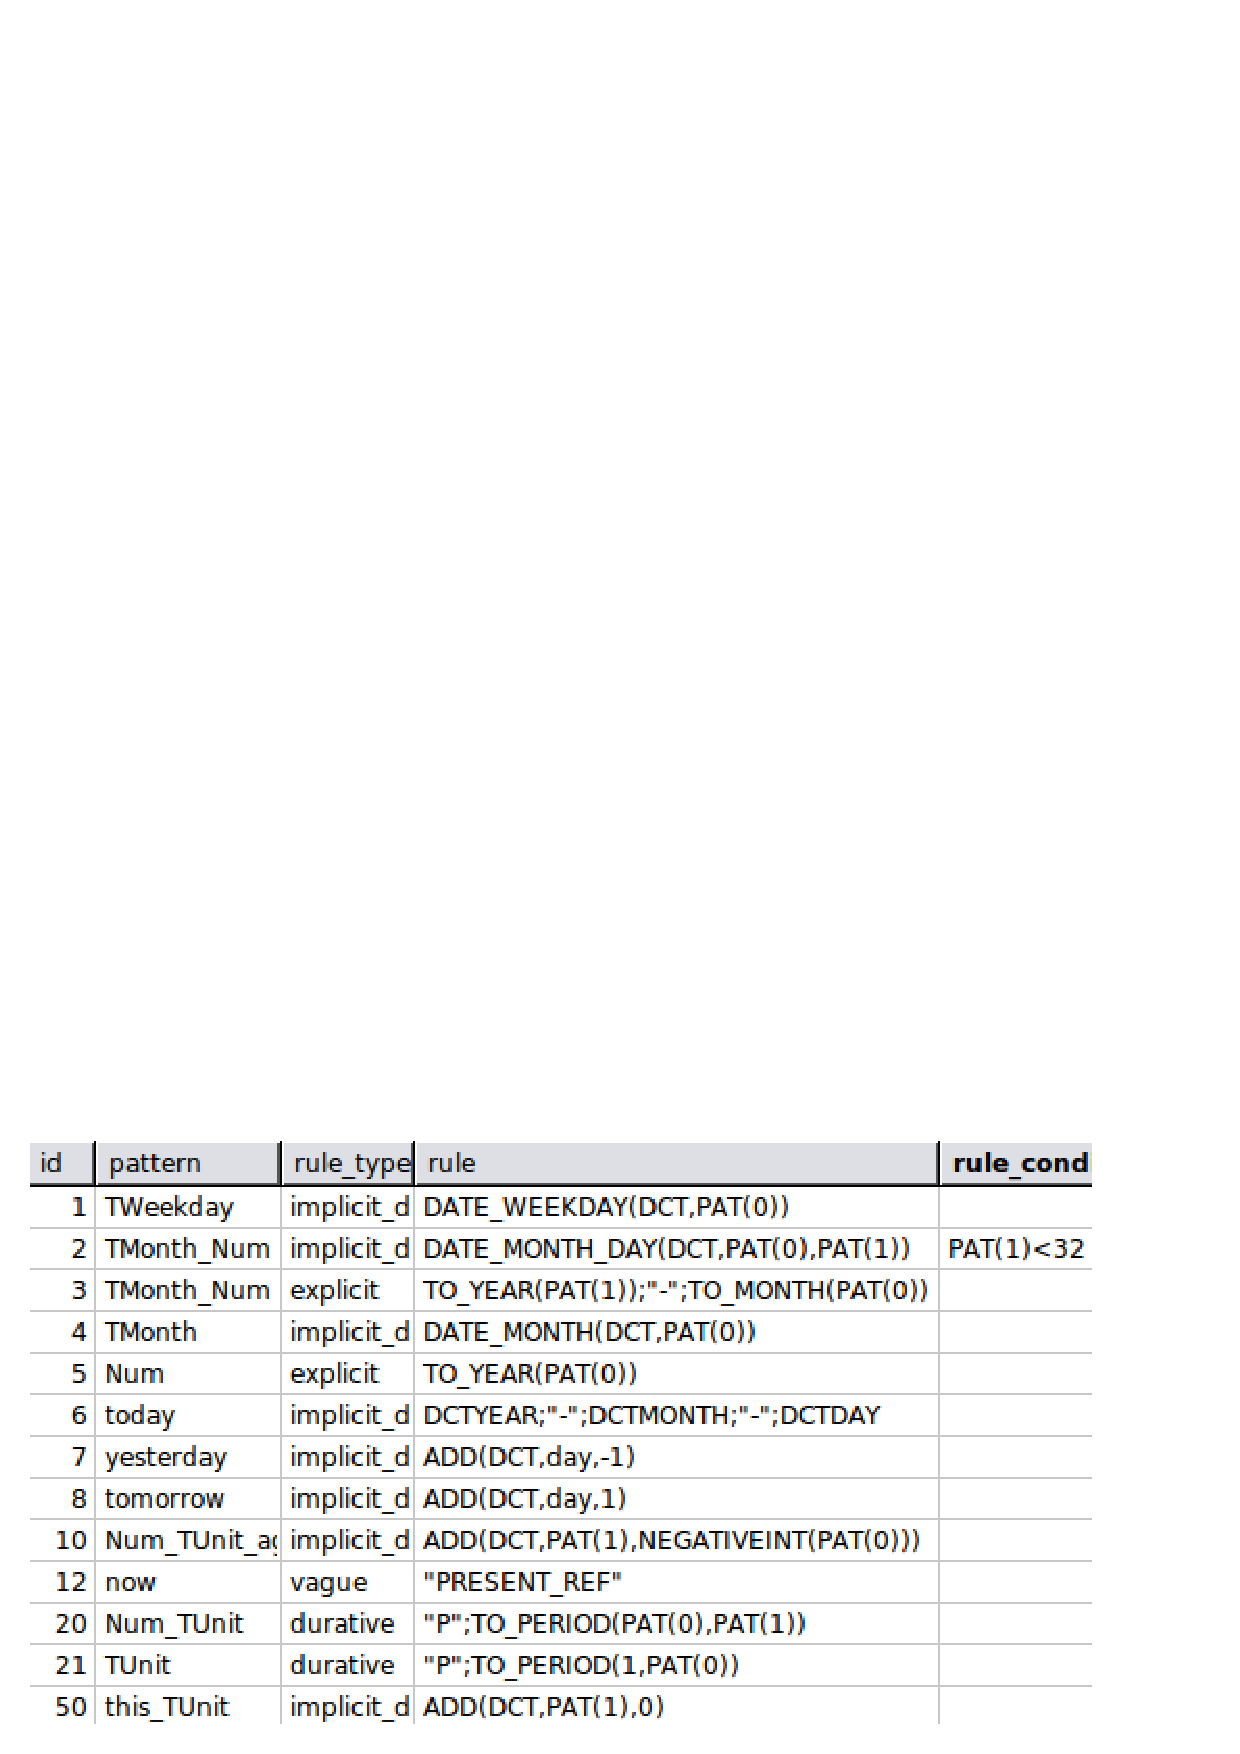
\includegraphics[width=0.5\textwidth,clip]{eps/screenshot.pdf}
  \caption{Snapshot of rules; here, the \textit{token()} function is \textit{PAT()}.}
  \label{fig:rules}
  \end{center}
\end{figure}

TIMEN and TIMEN\_CONSUMER have been made available on-line, at the TIMEN website\footnotemark[\value{footnote}].
This website also serves as an interface for the community integration of the resource explained in the next section.


\subsection{Community Integration}
\label{community}

% INCORPORATE SOME KIND OF FEEDBACK TO JUDGE NEW RULE EFFICACY
% AVAILABLE CORPUS TEST AND IF THERE IS NO IMPROVEMENT NEW CORPUS SUBMISSION (EXAMPLES)
In this section, we describe how we manage the collaborative community-led management of a normalisation rule base.

Our approach to timex interpretation relies on the premise that the normalisation problem can only be completely solved with some application of hand-crafted rules. A universal tool needs a hugely comprehensive rulebase; one that cannot be constructed in a short amount of time or by a small group of people. To overcome this, TIMEN's collaborative rule repository can be edited by any interested party.

Modification and addition of rules must be enabled in a way that ensures quality. Each rule includes an optional full TIMEX3 annotation that shows a timex in context and also its type and value. Using this, each rule can be verified. When a rule is to be modified or added, an included testing component verifies the rule set and highlights failing or broken rules.

We enable the community aspect of TIMEN with a website that lets users submit/modify rules, using:

\begin{itemize}
\item \textbf{Rule ID:} a descriptive name for the rule.
\item \textbf{Rule code:} the encoded rule. % pattern, rule, conditions
\item \textbf{Example timex:} a sentence containing a TIMEX3 tag, that is normalisable using the rule. The normalised text and the annotated TIMEX3 value are compared to validate the rule's operation.
\item \textbf{Language:} a two-letter language code representing which language rulebase this entry is destined for.
\item \textbf{Rule name:} (optional) free text describing the rule.
\end{itemize}

\begin{figure}
\centering
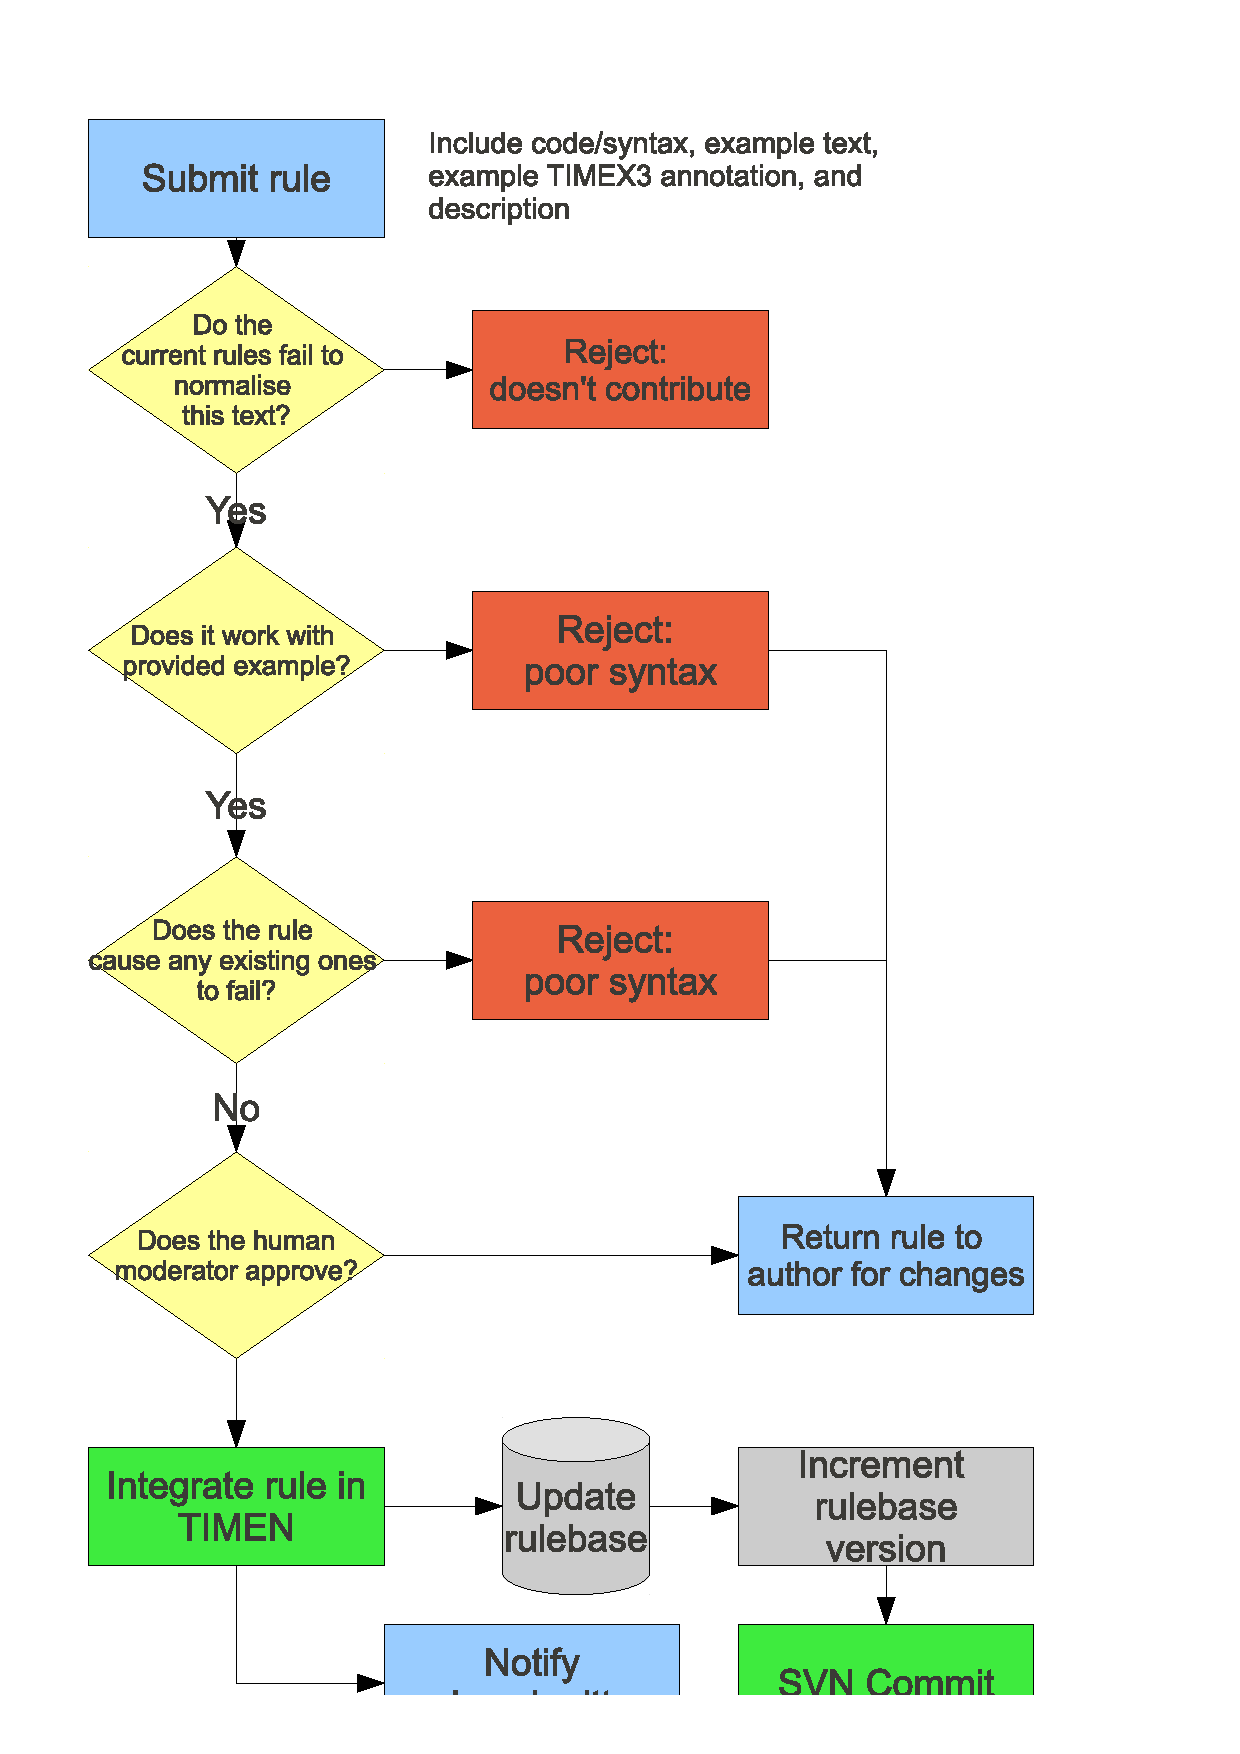
\includegraphics[width=0.5\textwidth,clip]{eps/rule-submission-process.pdf}
\caption{Moderation process for adding new entries to TIMEN.}
\label{fig:moderation}
\end{figure}

We manually moderate new rules, but they will be automatically rejected if the rule reduces performance on a predefined test set, the rule does not work for the example timex or the example can already by normalised by the existing ruleset. The website used for this process is based on Wordpress, and new rules use the ``posts" mechanism, allowing us to re-use the moderation and comments facilities without building a new management system from scratch. The process for moderating and accepting new rules is detailed in Figure~\ref{fig:moderation}.

TIMEN also includes an update mechanism which can automatically download new rules and knowledge base entries into an existing installation.


\section{Evaluation}
\label{evaluation}

In this section, we evaluate TIMEN using an existing dataset that is commonly used for normalisation evaluation, and using a newly created corpus which we also introduce. This first evaluation of TIMEN has two primary goals: (i) measuring the performance of TIMEN itself over gold TimeML annotated data, and (ii) measuring whether or not the application of TIMEN over currently available timex processing systems leads to an improvement of their performance in normalisation.

\subsection{Development Data}
The evaluation in this chapter is intended to reflect results based on resources that other state-of-the-art normalisation systems have. Therefore, the development dataset consists of the TimeBank and AQUAINT TimeML corpora and the TempEval-2 English training TIMEX3 annotations.

\subsection{TIMEX3 Evaluation Datasets}
Evaluations are in two datasets the TempEval-2 test dataset and a newly created dataset (TimenEval).
Both TIMEN and, theoretically, also the available systems, have developed their normalisation rule sets using the TempEval-2 training dataset, a part of TimeBank 1.2 corpus\footnote{\scriptsize \url{http://timeml.org/site/timebank/}}.

\subsection{New Dataset: TimenEval}
For TIMEN evaluation, not only do we evaluate using a well-known prior dataset, we also create and include a new resource for timex normalisation evaluation.
Most existing systems have been built using the same datasets for development -- TimeBank, AQUAINT and TempEval-2.
We therefore generated new data to see how the systems (including TIMEN) perform on unseen timexes. The dataset is intended to focus on diversity of both expression of time (e.g. input text) and intensional value (manifested by the resulting normalised timex). To this end, it contains a significant amount of non-newswire material.

For this new dataset (TimenEval), we include new data not been seen by the authors of any existing systems. The total data, we developed a set of over 200 TIMEX3s. We took care to achieve a good distribution of dates, times, durations and sets. Two annotators manually selected English test documents from the TAC KBP Source Collection\footnote{\scriptsize LDC ref. LDC2010E12, \emph{TAC 2010 KBP Source Data}.}. Annotations were validated both with the CAVaT TimeML checking tool~\cite{derczynski2010cavat} and also via XML Schema. Table \ref{tab:Data} summarizes the statistics of the data used for testing including the inter-annotator agreement (IAA). Lenient and strict extent IAA were 0.98 and 0.93 respectively, with strict+value IAA of 0.91. For all TIMEX3 attributes (inluding \texttt{quant}, \texttt{mod}, \texttt{freq}, \texttt{type} and \texttt{value}), we reached 0.85 IAA.

\begin{table} [htb]
\begin{footnotesize}
\begin{center}
\begin{tabular} {lcclc}
  \hline\rule{-2pt}{8pt}
  {\bf Test set} & {\bf Docs} & {\bf Words} & {\bf Timexes} & {\bf IAA}\\
  \hline\rule{-2pt}{8pt}
  {\bf TempEval-2} 	& 9	&  5.5k 	& 81  & 0.89\\
  {\bf TimenEval}		& 9	&  7.9k 	& 214  & 0.91\\
%date(69), duration(8), time(4), set(0)
  \hline
\end{tabular}
\caption{Corpus creation information, comparing the TempEval-2 evaluation set with TimenEval. IAA is for strict extent recognition and value.}
\label{tab:Data}
\end{center}
\end{footnotesize}
\end{table}

The major difference with the TempEval-2 dataset is in the distribution of TIMEX3 types. TempEval-2's test data set had only 6 \texttt{TIME}s and no \texttt{SET}-type timexes; TimenEval improves notably on both these counts. Statistics regarding timex type in TimenEval are shown in Table~\ref{tab:timeneval-type}. The TimenEval TIMEX3 dataset is available at \url{http://www.timen.org/}.

\begin{table}
\begin{center}
\begin{tabular}{  l  r  r  r  }
\hline
\textbf{TIMEX3 type} & \textbf{Frequency} & \textbf{Proportion} \\
\hline
DATE & 121 & 56.5\% \\
TIME & 43 & 20.1\% \\
DURATION & 34 & 15.9\% \\
SET & 16 & 7.48\% \\
\hline
Total & 214 &  \\
\hline
\end{tabular}
\caption{Distribution of TIMEX3 type}
\label{tab:timeneval-type}
\end{center}
\end{table}


\subsection{TIMEN Performance}

For the first goal, we run TIMEN over the gold annotations of both the test set in the TempEval-2 evaluation and our newly created dataset.
Our initial evaluation measures intrinsic normalisation accuracy using gold-standard timex annotations.
Table \ref{tab:TIMEN} shows the obtained results.

\begin{table} [htb]
\begin{footnotesize}
\begin{center}
\begin{tabular} {lcc}
  \hline\rule{-2pt}{8pt}
  {\bf Test set} &  {\bf Recall} &{\bf Normalisation accuracy}\\
  \hline\rule{-2pt}{8pt}
  {\bf TempEval-2}  	& (1.0)	& 0.90\\
  {\bf TimenEval}	& (1.0)	& 0.68\\
  \hline
\end{tabular}
\caption{TIMEN performance. Recall is full to reflect that these results apply to all timexes in the dataset, and we are not just performing at these rates over a selected recognised subset, for comparison with TempEval-2 scorings. TIMEN does not do any timex recognition.} 
\label{tab:TIMEN}
\end{center}
\end{footnotesize}
\end{table}

So far, the current TIMEN version has only 76 rules covering only the most common timexes.
With this young and incomplete rule set we obtained high results -- 90\% in TempEval-2 and 68\% in TimenEval.

A priori, these results seem comparable to those obtained by the best normalisation system in TempEval-2 (e.g., HeidelTime: 0.85).
However, because HeidelTime only recognised 86\% of all timexes in the TempEval-2 test set, that 0.85 means that HeidelTime normalised correctly only the 86\% of timexes it was exposed to.
Results are not thus comparable and we can therefore only assert with full certainty that HeidelTime normalised correctly at least 0.73 (0.85$*$0.86) out of the total timexes.

To conduct a fair, comparable and rigorous evaluation, we carried out the second experiment detailed below, in which each system is evaluated and combined with TIMEN to detect if TIMEN gives an improvement in the normalisation performance -- which is its goal.

\subsection{Using TIMEN with other systems}

For the second goal, measuring the performance change TIMEN offers over other systems' normalisation components, we compare the performance of three other publicly-available state of the art timex processing systems (i.e., TIPSem, TERNIP, HeidelTime), firstly with their own normalisation code's TIMEX3 values and secondly with those supplied by TIMEN. Specifically, we run these systems over a dataset and measure their own normalisation performance. Then, we substitute their normalisation component with TIMEN, and re-evaluate, using their recognised timex extents as input. This is made possible by TIMEN\_CONSUMER's support for operation as a drop-in component that can take existing TIMEX3 annotations and change/add only the attributes relevant to normalisation.

We carried out the described evaluation over the TempEval-2 test data and over a newly annotated documents which have neither been used to build the evaluated systems nor TIMEN. Tables \ref{tab:TE2} and \ref{tab:timeneval} show the results obtained in each dataset. Performance is scored as in TempEval-2; that is, extents is the F1 measure of strict extent detection, and the normalisation scores are the percentage of correct TIMEX3 values determined for the subset of detected timexes.


\begin{table*} [htb]
\begin{footnotesize}
\begin{center}
\begin{tabular} {lcccr}
  \hline\rule{-2pt}{8pt}
  {\bf System} & {\bf Extents} & {\bf Internal norm.} & {\bf TIMEN norm.} & {\bf Err. reduction}\\
  \hline\rule{-2pt}{8pt}
  {\bf TIPSemB} 	& 0.94	& 0.83	& 0.89	& +35\% \\
  {\bf HeidelTime} 	& 0.86	& 0.94	& 0.94  & +0\%  \\
  {\bf TERNIP} 		& 0.85 	& 0.76	& 0.92	& +66\% \\
  \hline
\end{tabular}
\caption{Systems evaluation over TempEval-2 test dataset} \label{tab:TE2}
\end{center}
\end{footnotesize}
\end{table*}
a
Results for TempEval-2 data are shown in Table~\ref{tab:TE2}. Given timexes with extents determined by each system, TIMEN performs significantly better than built-in normalisation components in all cases except HeidelTime's, where it matches performance. Bear in mind that HeidelTime has been actively developed long after TempEval-2 with access to this dataset, just as TIMEN has.


\begin{table*} [htb]
\begin{footnotesize}
\begin{center}
\begin{tabular} {lcccr}
  \hline\rule{-2pt}{8pt}
  {\bf System} & {\bf Extents} & {\bf Internal norm.} & {\bf TIMEN norm.} & {\bf Err. reduction}\\
  \hline\rule{-2pt}{8pt}
  {\bf TIPSemB} 		& 0.51	& 0.57	& 0.67	& +23\%  \\
  {\bf HeidelTime} 		& 0.70	& 0.72	& 0.74	& +7.1\% \\
  {\bf TERNIP} 			& 0.73	& 0.70	& 0.72	& +6.6\% \\
  \hline
\end{tabular}
\caption{Systems evaluation over TimenEval} \label{tab:timeneval}
\end{center}
\end{footnotesize}
\end{table*}

Results on the TimenEval dataset are given in Table~\ref{tab:timeneval}. This evaluation treats normalisation equally, as no system has seen the dataset before. Again, TIMEN provides a significant performance boost in all cases, even over HeidelTime's normalisation. It is interesting to see an increase here, as HeidelTime uses an integrated recognition and normalisation ruleset, and might not be expected to recognise timexes that it could not normalise. TIPSemB's low results are due to the variable quality of the text in the dataset. Timex annotations are not as structured as those in TempEval-2, but instead include some technical noise (e.g. newline breaks in timexes). This makes it difficult for the integrated model to recognise timexes. To improve this, re-training on informal / unformatted text is required. Rule-based systems do not have this kind of limitation in new genres.

\subsection{Error analysis and discussion}

Development of the gold dataset was hard, particularly regarding variation in available standards. ISO-8601, TIDES TIMEX2 and TimeML TIMEX3 all contribute to the normalisation value format. Example cases include the treatment of negative dates, where (for historic reasons) TIDES and ISO-8601 diverge; for date delimitation, where ISO-8601 permits a variety of schemes, TIMEX2 and TIMEX3 are non-specific, but all existing tools and resources use hyphenated dates; and treatment of generic temporal pronouns, such as in \emph{``this time"}. Our experience is that future work on clarifying and improving upon the TimeML TIMEX3 guideline is warranted, perhaps as a contribution for ISO-TimeML.

Some systems do not retain enough information about temporal context. For example, when talking about the third quarter of 1989 with a DCT of 1989, HeidelTime always interprets \emph{``a year ago"} as 1988 (instead of 1988-Q3). In the evaluation datasets, TIMEN normalised this kind of expression correctly.

Words that describe times briefly using contextual clues were also hard to normalise, as in \emph{``Why 10am? Why not twelve, or two, or four?"}. Complex cases were also difficult, such as with \emph{``Every 2 weeks at 16:00 on Saturday"} from eng-NG-31-142881-10102642.tml.

Finally, unusual phrases were difficult to interpret. These should be the easiest category of all to add rules for to a communal resource. They include items such as \emph{``Purim"}, \emph{``the intercalary day"} and \emph{``Mid-Autumn Festival"}.
Gazetteers and other lists of holiday events contain explicit rules for resolving a holiday name to a date, given a year. Combing through these resources and adding them to TIMEN will improve our normalisation coverage.

\section{Conclusion}

We have presented an open and independent state-of-the-art tool for timex normalisation: TIMEN.

Its performance results show improvement in normalisation over recent approaches, demonstrating that TIMEN is a new effective resource for normalisation regardless of timex recognition approach.
Furthermore, it removes the cost of re-developing a timex normalisation system.
This saves time and favors the improvement of the resource via community contribution and evaluation. 
This makes TIMEN an extensible and reusable tool, finally overcoming the boundary that all previous timex normalisation systems have suffered from at the end of their development.

\subsection{Future Work}
Regarding future work, the central effort is the ongoing extension and refinement of TIMEN's rule base. We encourage community participation in this. 
Future work will improve performance through building up the rule base, making TIMEN a viable long-term choice for timex normalisation.

We plan to extensively evaluate TIMEN over more data and publish a high-coverage normalisation resource not limited to English but including other languages such as Spanish, Chinese, Italian and Danish. As the TempEval-2 dataset includes gold standard examples in many languages, initial construction of these rule bases can be data-driven. The nature of our framework reduces the barrier to adding new languages and to contribute to the normalisation of those languages, as it uses only a simple purpose-built rule syntax.


\section*{Acknowledgments}
Leon Derczynski would like to acknowledge the UK Engineering and Physical Science Research Council's support in the form of a doctoral studentship.
This paper has been also supported by the Spanish Government, in projects: {\scriptsize TIN-2009-13391-C04-01}, {\scriptsize TIN2010-14860}, {\scriptsize PROMETEO/2009/119}, and {\scriptsize ACOMP/2011/001}.

%\nocite{*}


\bibliographystyle{lrec2006}
\bibliography{bib} 

\end{document}

